\documentclass{article}
%
% Demo of the mcode package from 
% http://www.mathworks.co.uk/matlabcentral/fileexchange/8015-m-code-latex-package
% Updated 06 Mar 2014
%

\usepackage{graphicx}
\usepackage{wrapfig}
\usepackage{mathtools}
\usepackage{mathrsfs}
\usepackage{enumitem}
\usepackage{pdflscape}
\graphicspath{ {images/} }

\usepackage{float}
% load package with ``framed'' and ``numbered'' option.
\usepackage[framed,numbered,autolinebreaks,useliterate]{mcode}

% something NOT relevant to the usage of the package.
\usepackage{url}
\setlength{\parindent}{0pt}
\setlength{\parskip}{18pt}


% //////////////////////////////////////////////////

\begin{document}

\title{Homework 8 - Optimal Control Systems}
\author{Erivelton Gualter dos Santos, 2703806}
\date{}

\maketitle 

\section{LQR problem}
\subsection*{Time-varying and Steady-state LQR - problems \textit{a} and \textit{b}}

Figure \ref{states1} compares the states for a Time-Varying LQR control approach with a Steady-state LQR. The responses are really close to each other with a root-mean-square (RMS) level of $0.0015$ and $0.0221$.
\begin{figure}[H] 
\centering
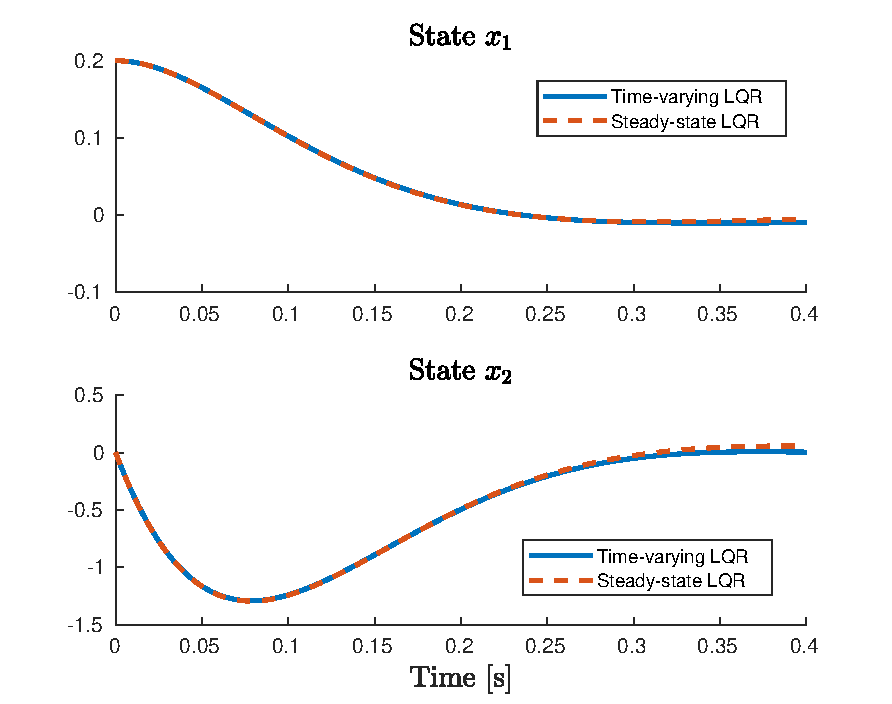
\includegraphics [width=4in]{states1} \label{states1}
\caption{States for time-varying and Steady State LQR.}
\end{figure}

\begin{figure}[H] 
\centering
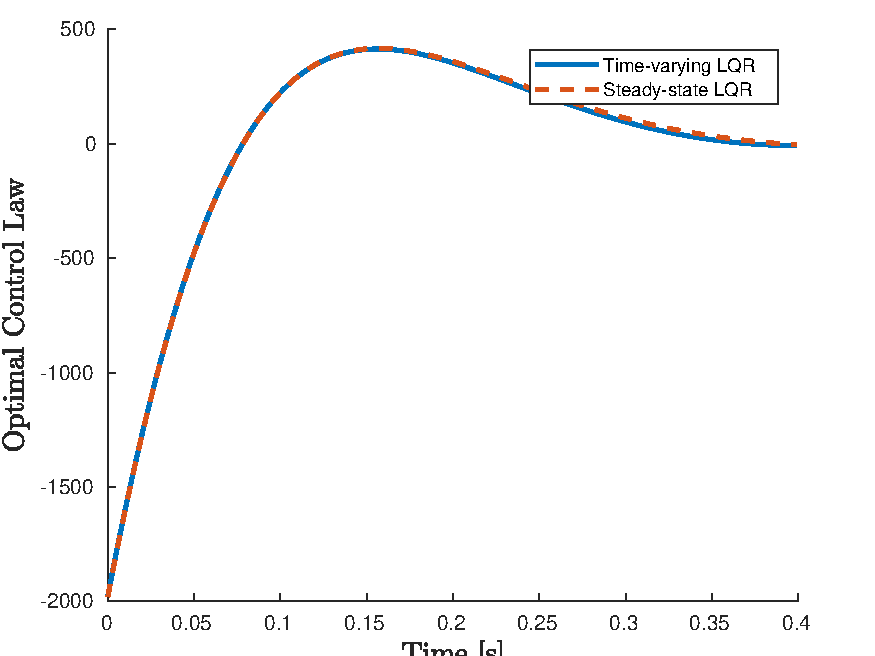
\includegraphics [width=4in]{control1} \label{control1}
\caption{States for time-varying and Steady State LQR.}
\end{figure}

\begin{figure}[H] 
\centering
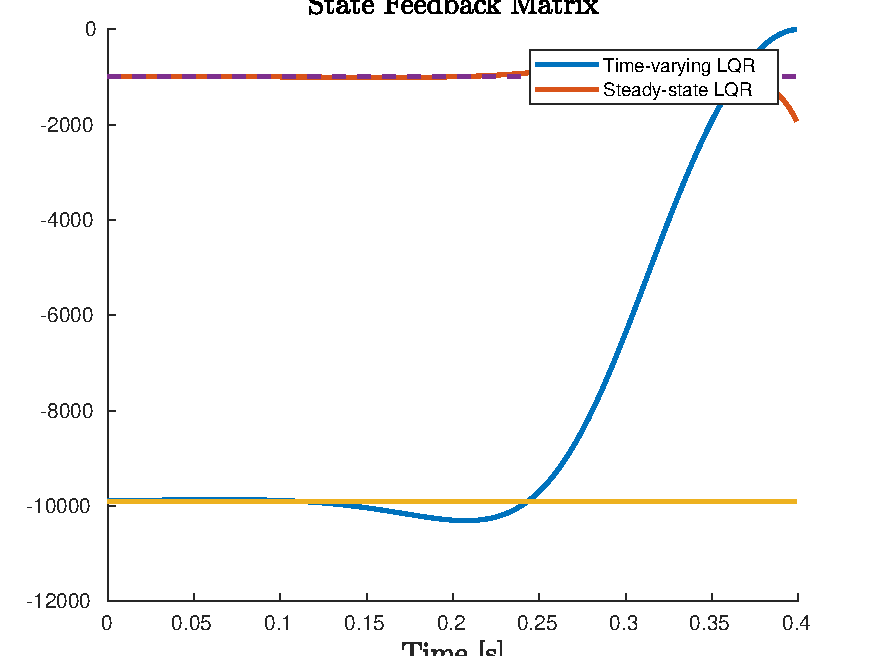
\includegraphics [width=4in]{gain1} \label{gain1}
\caption{States for time-varying and Steady State LQR.}
\end{figure}

\pagebreak
The total cost for the time-varying and steady state also is similar. Figure 4 shows the cost plot which results in the cost correspond to $2.0189$ and $2.0194$.

\begin{figure}[H]
\centering
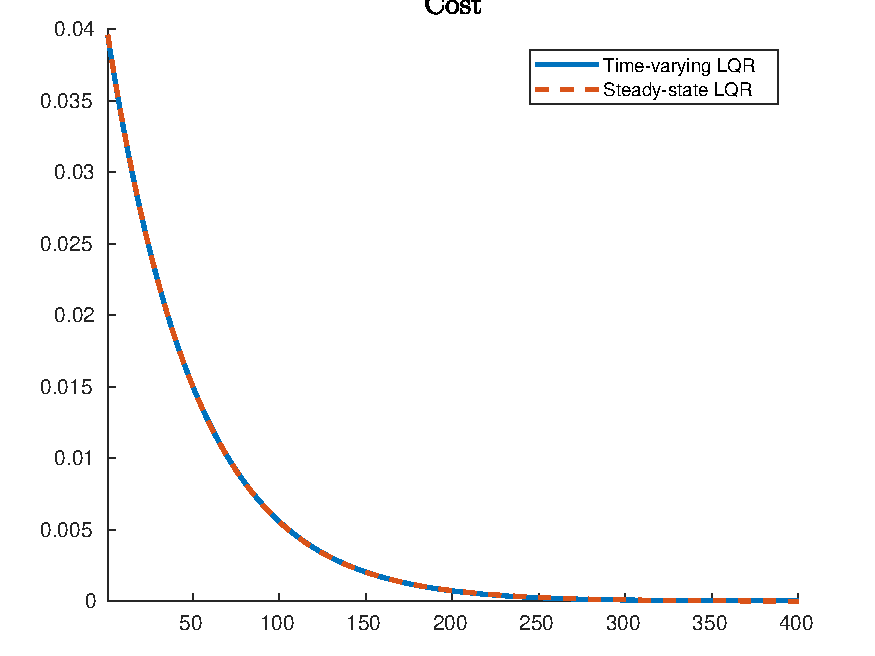
\includegraphics [width=4.5in]{cost1}
\caption{States for time-varying and Steady State LQR.}
\end{figure}



\subsection*{Time-varying and Steady-state LQR for tf=0.2s}

\begin{figure}[H] 
\centering
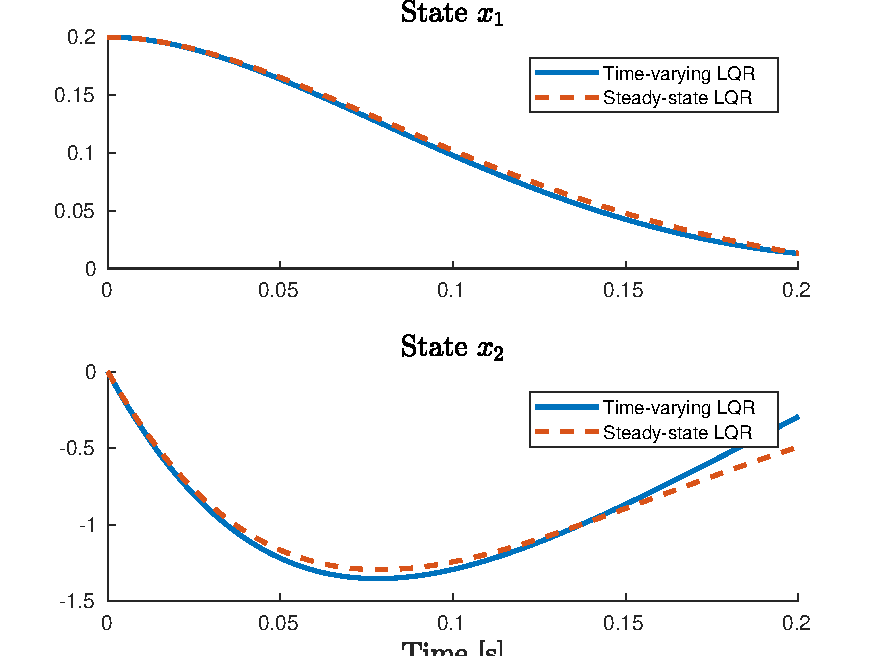
\includegraphics [width=4in]{states2} \label{states1}
\caption{States for time-varying and Steady State LQR.}
\end{figure}

\begin{figure}[H] 
\centering
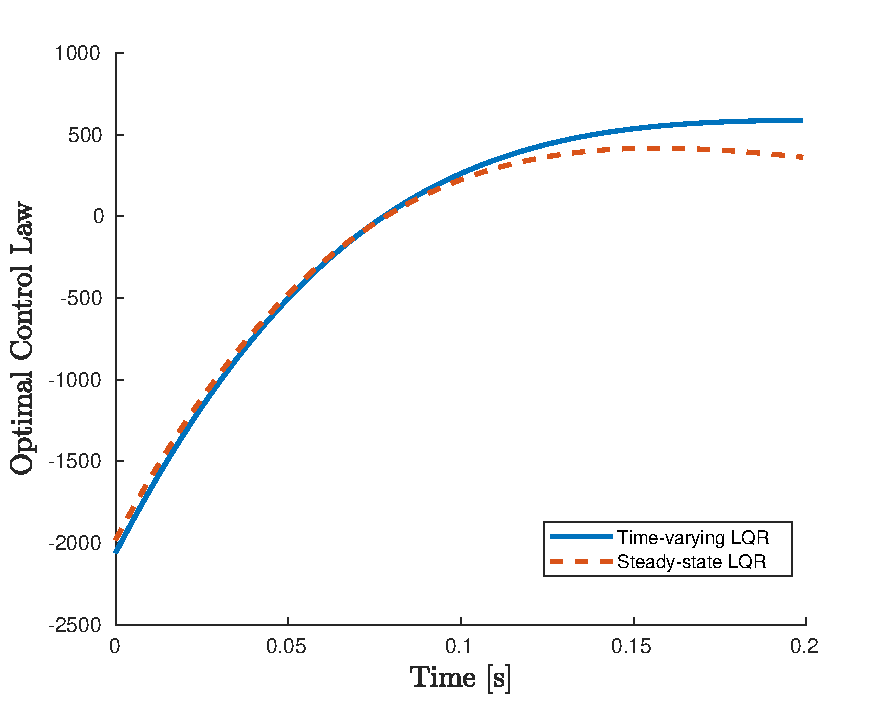
\includegraphics [width=4in]{control2} \label{control1}
\caption{States for time-varying and Steady State LQR.}
\end{figure}

\begin{figure}[H] 
\centering
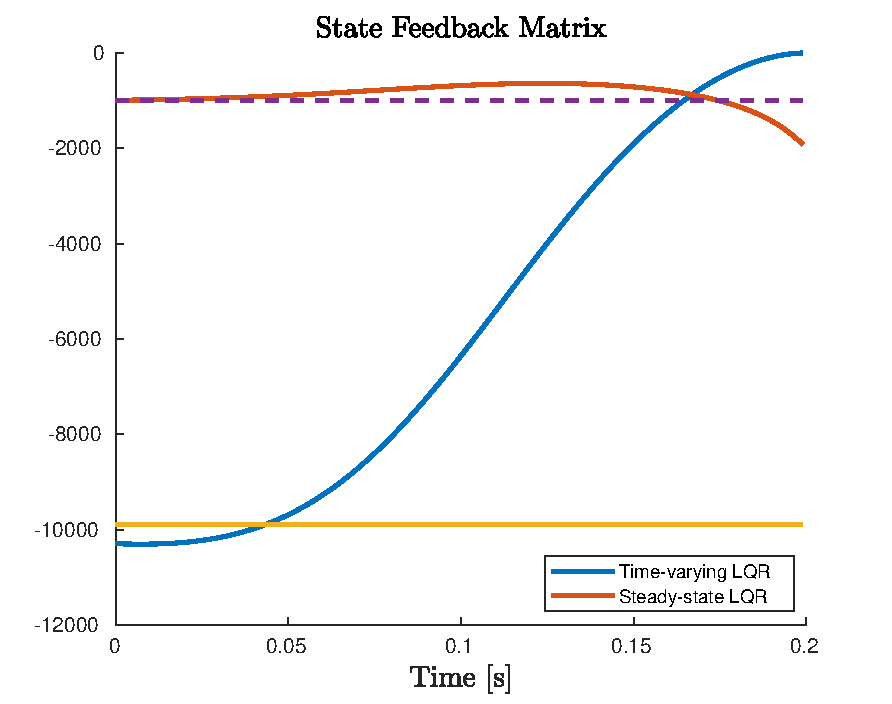
\includegraphics [width=3.5in]{gain2} \label{gain1}
\caption{States for time-varying and Steady State LQR.}
\end{figure}

The total cost for the time-varying and steady state also is similar. Figure 4 shows the cost plot which results in the cost correspond to $2.0302$ and $1.9828$.

\begin{figure}[H]
\centering
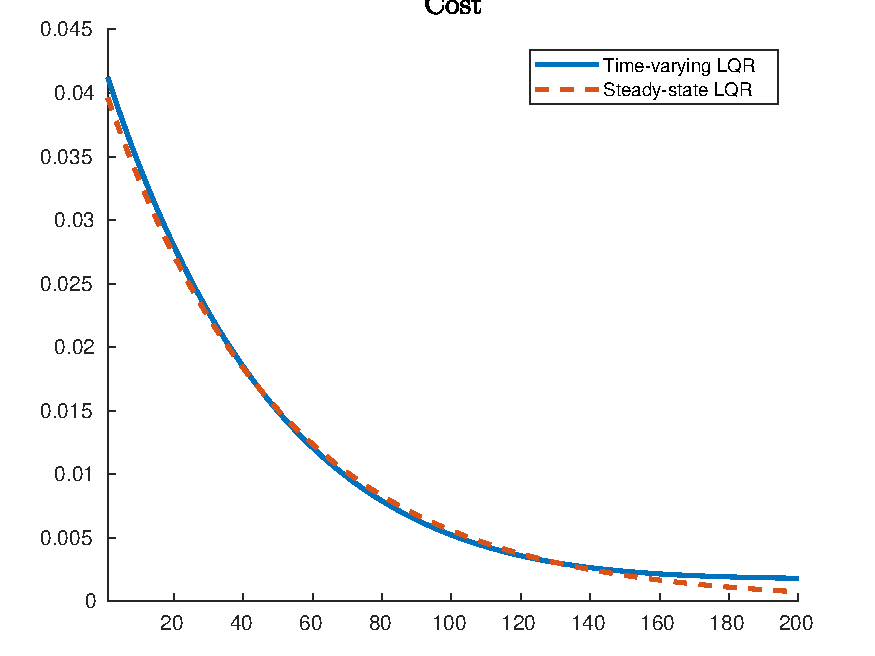
\includegraphics [width=3.5in]{cost2}
\caption{States for time-varying and Steady State LQR.}
\end{figure}

\subsection*{Hamiltonian matrix approach}

Figure 9 compares the states for a Steady-state LQR used in the problem b with the Hamiltonian matrix approach. The responses are really close to each other with a root-mean-square (RMS) level of $0.0004$ and $0.0044$.

\begin{figure}[H] 
\centering
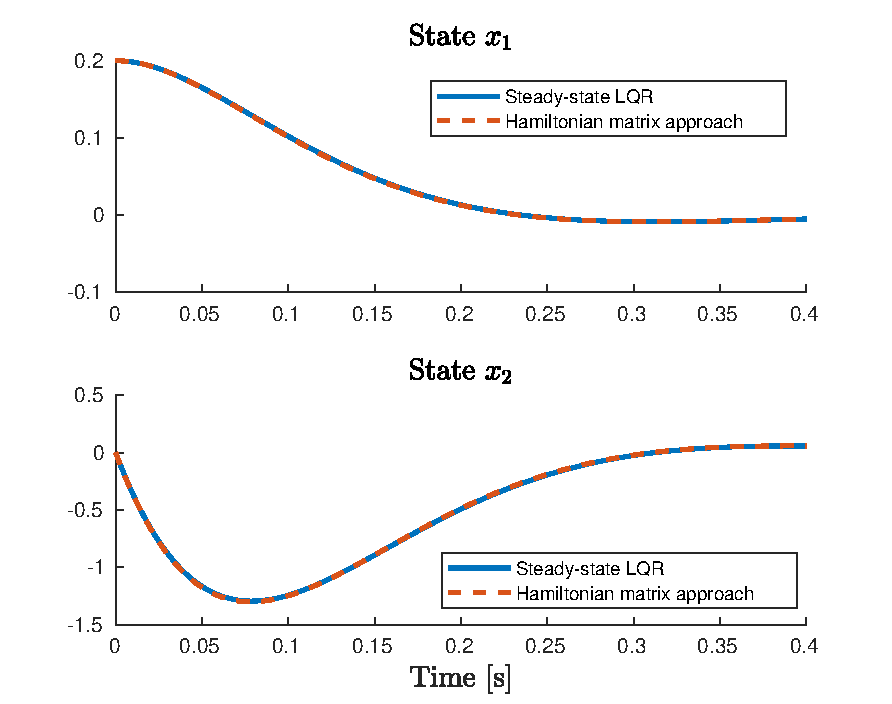
\includegraphics [width=3.5in]{states3} \label{states3}
\caption{States for time-varying and Steady State LQR.}
\end{figure}

\begin{figure}[H] 
\centering
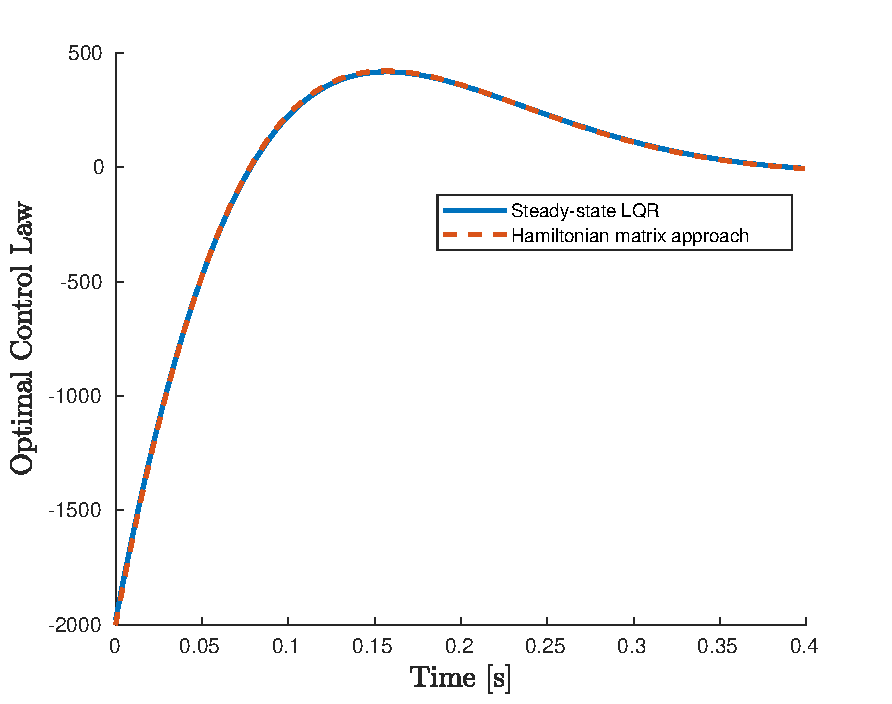
\includegraphics [width=3in]{control3} \label{control3}
\caption{States for time-varying and Steady State LQR.}
\end{figure}

\begin{figure}[H] 
\centering
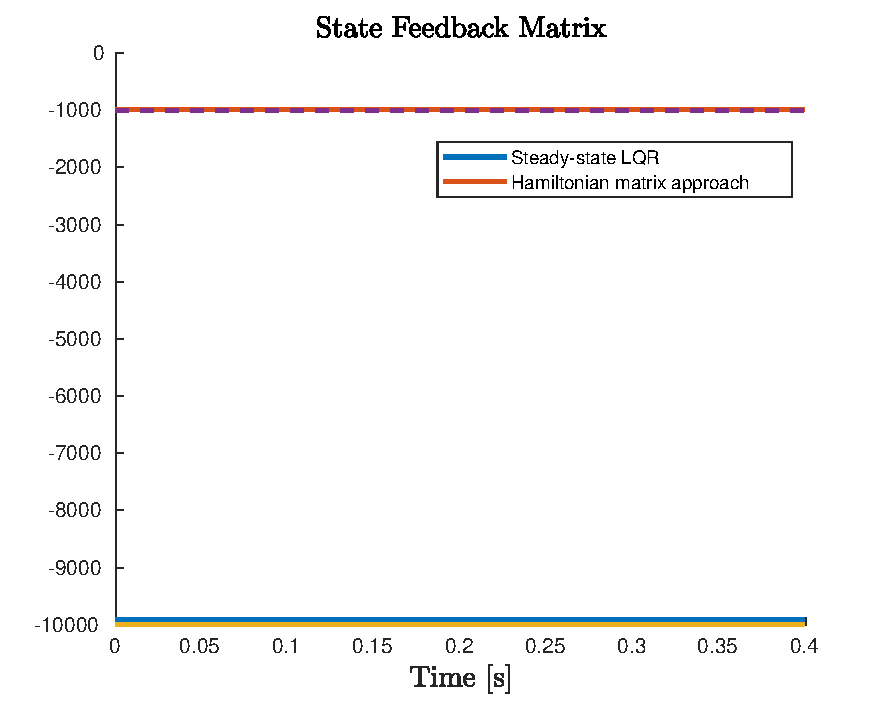
\includegraphics [width=3.5in]{gain3} \label{gain3}
\caption{States for time-varying and Steady State LQR.}
\end{figure}

The total cost for the time-varying and steady state also is similar. Figure 4 shows the cost plot which results in the cost correspond to $2.0302$ and $1.9828$.

\begin{figure}[H]
\centering
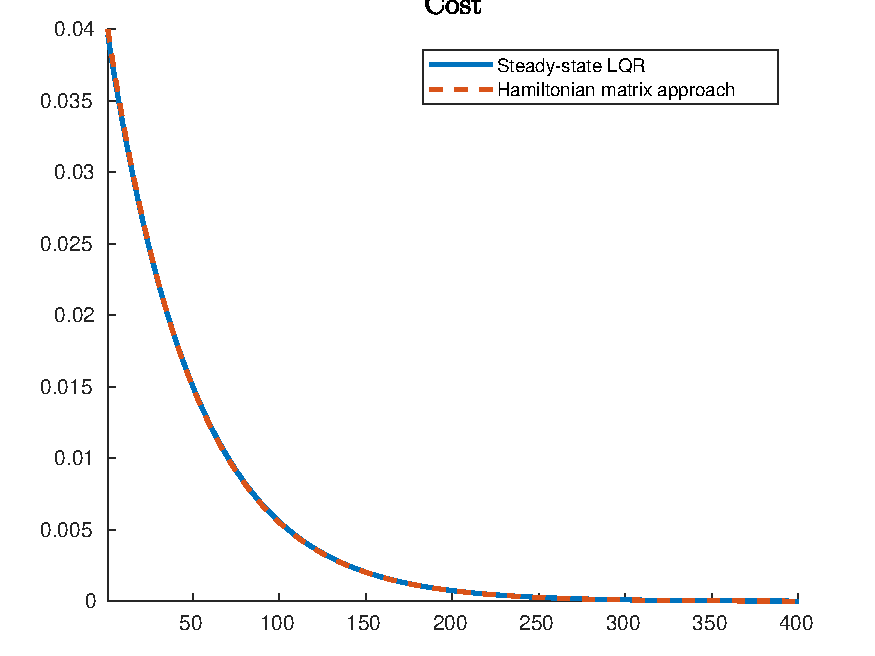
\includegraphics [width=3.5in]{cost3}
\caption{States for time-varying and Steady State LQR.}
\end{figure}

\section{Variational Problem}
Consider the following system and cost function with fixed final time:
\begin{equation}
x' = -x + u
\end{equation}
and cost function as:
\begin{equation}
J = \int e^u + (1-x)^2  e^{-t} dx 
\end{equation}
\subsection{Hamiltonian}
\begin{eqnarray*}
\begin{split}
\mathcal{H} &= g +p^Ta \\
&= (e^u+(1-x)^2)e^{-t})+p(-x+u)
\end{split}
\end{eqnarray*}

\subsection{Euler-Lagrange equations}

%From the derived variation equation in Kirk's book:
%\begin{eqnarray*}
%\begin{split}
%\delta J(x^*,\delta x) &= \left[\frac{\partial g}{\partial \dot{x}} (x^*(t_f),\dot{x}^*(t_f),t_f) \right]\delta x_f \\
%&+ \left[ g(x^*(t_f),\dot{x}^*(t_f),t_f) - \left[\frac{\partial g}{\partial \dot{x}} (x^*(t_f),\dot{x}^*(t_f),t_f) \right]\dot{x}^*(t_f) \right]\delta x_f \\
%&+ \int_{t_o}^{t_f} \lbrace \frac{\partial g}{\partial x}(t_f),\dot{x}^*(t_f),t_f) - \frac{d}{dt}\left[\frac{\partial g}{\partial \dot{x}} (x^*(t_f),\dot{x}^*(t_f),t_f) \right]  \rbrace \delta x(t) dx
%\end{split}
%\end{eqnarray*}

As the problem is the problem has fixed final time:

\begin{eqnarray*}
\begin{split}
\frac{\partial h}{\partial x} = -2(1-x)e^{-t}-p \\
\frac{\partial h}{\partial t} = -(1-x)^2e^{-t} = 0
\end{split}
\end{eqnarray*}

For $\delta x(t_f)=0$, we have:
\begin{eqnarray*}
\begin{split}
\frac{\partial h}{\partial x} - p &= -2(1-x)e^{-t}-p - p \\
&= (1-x)e^{-t}+p = 0
\end{split}
\end{eqnarray*}

For $\delta t_f=0$, we have:
\begin{eqnarray*}
\begin{split}
\mathcal{H}+\frac{\partial h}{\partial t} &= (e^u+(1-x)^2)e^{-t})+p(-x+u) -(1-x)^2e^{-t} \\
&= e^u+p(-x+u) = 0
\end{split}
\end{eqnarray*}

The necessary conditions are:
\begin{eqnarray}
\begin{split}
\dot{x}^*(t) = \frac{\partial \mathcal{H}}{\partial p} &= -x+u \\
\dot{p}^*(t) = -\frac{\partial \mathcal{H}}{\partial x} &= 2(1-x)e^{-t}+p \\
0 = \frac{\partial \mathcal{H}}{\partial u} &= e^u+p
\end{split}
\end{eqnarray}

From the necessary conditions, we can $u(t)$ can be written as a function of p: 
\begin{eqnarray*}
u = \ln(-p)
\end{eqnarray*}

In order to solve this problem, first we need to create the array time ($t_o$ to $t_f$) with a defined $dt$ time step simulation to solve the problem interactively. Then, find $p$ from the necessary condition equations ($\dot{p}^*$)  using Euler Integration method with the desired initial conditions. Then, find the control input for this interaction and find the next state using the Euler Integration method of the system. 

 
\begin{lstlisting}
% Book: Optimal Control Theory: An introduxtion by Donald E. Kirk
%
% Erivelton Gualter, 03/26/2018

clear all; close all;

% Plant
A = [0 1; 0 -0.02];
B = [0 ; 0.02];

% Simulation Parametes
X0 = [0.2; 0];  % Initial States
tf = 0.4; %0.2; % Final time [s]
dt = 1e-3;      % Sampling time
N = tf/dt+3;
t = 0:dt:tf;

% LQR Parameters
H = zeros(size(A));
Q = [1 0; 0 0];
R = 1e-8;

%% A, B and C probelm %%%%%%%%%%%%%%%%%%%%%%%%%%%%%%%%%%%%%%%%%%%%%%%%%%%%%
[Ad, Bd] = c2d(A,B, dt);
N = tf/dt+2;
P(:,:,1)= eye(2);    
for k=2:N-1 % Backwards loop to find P and K
    S = R + Bd'*P(:,:,k-1)*Bd;
    F(:,:,N-k) =  -( inv(S) * Bd' * P(:,:,k-1) * Ad );
    P(:,:,k) = (Ad + Bd*F(:,:,N-k))'*P(:,:,k-1)*(Ad + Bd*F(:,:,N-k)) + F(:,:,N-k)'*R*F(:,:,N-k) + Q;
end

X1 = X0;
X2 = X0;
for k=1:N-2  % Simulate systen using Euler Integration

    % Time varying 
    u1(k) = F(:,:,k)*X1(:,k);
    
    XD1 = A*X1(:,k) + B*u1(k);
    X1(:,k+1) = X1(:,k) + XD1*dt;
    
    % Steady-stae
    Pss = dare(Ad,Bd,Q,R);
    S = R + Bd'*Pss*Bd;
    Fss = -( inv(S) * Bd' * Pss * Ad );
    u2(k) = Fss*X2(:,k);   
    
    XD2 = A*X2(:,k) + B*u2(k);
    X2(:,k+1) = X2(:,k) + XD2*dt;
end

% Performance Measure (calc cost)
Jt1 = 0;
Jt2 = 0;
for k=1:N-2
    J1(k) = X1(:,end)'*H*X1(:,end)/2 + (X1(:,k)'*Q*X1(:,k) + u1(k)*R*u1(k))/2;
    Jt1 = Jt1 + J1(k);
    
    J2(k) = X2(:,end)'*H*X2(:,end)/2 + (X2(:,k)'*Q*X2(:,k) + u2(k)*R*u2(k))/2;
    Jt2 = Jt2 + J2(k);
end

%%
close all
f1 = figure;
ax1 = subplot(211); hold on; plot(t, X1(1,:),'LineWidth',2); plot(t, X2(1,:),'--','LineWidth',2);
ax2 = subplot(212); hold on; plot(t, X1(2,:),'LineWidth',2); plot(t, X2(2,:),'--','LineWidth',2);
title(ax1, 'State $x_1$','Interpreter','latex','FontSize',14); 
title(ax2, 'State $x_2$','Interpreter','latex','FontSize',14);   
legend(ax1, 'Time-varying LQR', 'Steady-state LQR');
legend(ax2, 'Time-varying LQR', 'Steady-state LQR');
xlabel('Time [s]', 'Interpreter','Latex', 'FontSize',14);
saveFigureToPdf('fig1',f1);
    
f2 = figure; hold on;
tu = t(1:end-1);
plot(tu, u1,'LineWidth',2); plot(tu, u2,'--','LineWidth',2);
legend('Time-varying LQR', 'Steady-state LQR');
xlabel('Time [s]', 'Interpreter','Latex', 'FontSize',14);
ylabel('Optimal Control Law', 'Interpreter','Latex', 'FontSize',14);
saveFigureToPdf('fig2',f2);

f3 = figure; hold on;
F_plot1(:,:) = F(1,:,:); 
F_plot2(1,:) = Fss(1)*ones(1,length(F));
F_plot2(2,:) = Fss(2)*ones(1,length(F));
plot(t(1:end-1), F_plot1(1,:), t(1:end-1), F_plot1(2,:),'LineWidth',2);
plot(t(1:end-1), F_plot2(1,:), t(1:end-1), F_plot2(2,:),'--','LineWidth',2);
legend('Time-varying LQR', 'Steady-state LQR');
xlabel('Time [s]', 'Interpreter','Latex', 'FontSize',14);
title('State Feedback Matrix', 'Interpreter','Latex', 'FontSize',14);
saveFigureToPdf('fig3',f3);

f4 = figure; hold on;
plot(J1,'LineWidth',2); plot(J2,'--','LineWidth',2);
xlim([1 length(J1)]);
title('Cost', 'Interpreter','Latex', 'FontSize',14);
legend('Time-varying LQR', 'Steady-state LQR');

saveFigureToPdf('fig4',f4);

%% D Probelm %%%%%%%%%%%%%%%%%%%%%%%%%%%%%%%%%%%%%%%%%%%%%%%%%%%%%%%%%%%%%%
N = length(t);
X3 = X0;
for k=1:N-1

    K = care(A,B,Q,R);
    u3(k) = -inv(R)*B'*K*X3(:,k);
    
    XD3 = A*X3(:,k) + B*u3(k);
    
    X3(:,k+1) = X3(:,k) + XD3*dt;    
end

% Performance Measure (calc cost)
Jt3 = 0;
for k=1:N-2
    J3(k) = X3(:,end)'*H*X3(:,end)/2 + (X3(:,k)'*Q*X3(:,k) + u3(k)*R*u3(k))/2;
    Jt3 = Jt3 + J3(k);
end
%%
f5 = figure;
ax1 = subplot(211); hold on; plot(t, X2(1,:),'LineWidth',2); plot(t, X3(1,:),'--','LineWidth',2);
ax2 = subplot(212); hold on; plot(t, X2(2,:),'LineWidth',2); plot(t, X3(2,:),'--','LineWidth',2);
title(ax1, 'State $x_1$','Interpreter','latex','FontSize',14); 
title(ax2, 'State $x_2$','Interpreter','latex','FontSize',14);   
legend(ax1, 'Steady-state LQR',  'Hamiltonian matrix approach');
legend(ax2, 'Steady-state LQR',  'Hamiltonian matrix approach');
xlabel('Time [s]', 'Interpreter','Latex', 'FontSize',14);
saveFigureToPdf('fig5',f5);
    
f6 = figure; hold on;
tu = t(1:end-1);
plot(tu, u2,'LineWidth',2); plot(tu, u3,'--','LineWidth',2);
legend('Steady-state LQR',  'Hamiltonian matrix approach');
xlabel('Time [s]', 'Interpreter','Latex', 'FontSize',14);
ylabel('Optimal Control Law', 'Interpreter','Latex', 'FontSize',14);
saveFigureToPdf('fig6',f6);

f7 = figure; hold on;
gain = -inv(R)*B'*K;
F_plot3(1,:) = gain(1)*ones(1,length(F));
F_plot3(2,:) = gain(2)*ones(1,length(F));
plot(t(1:end-1), F_plot2(1,:), t(1:end-1), F_plot2(2,:),'LineWidth',2);
plot(t(1:end-1), F_plot3(1,:), t(1:end-1), F_plot3(2,:),'--','LineWidth',2);
legend('Steady-state LQR',  'Hamiltonian matrix approach');
xlabel('Time [s]', 'Interpreter','Latex', 'FontSize',14);
title('State Feedback Matrix', 'Interpreter','Latex', 'FontSize',14);
saveFigureToPdf('fig7',f7);

f8 = figure; hold on;
plot(J2,'LineWidth',2); plot(J3,'--','LineWidth',2);
xlim([1 length(J2)]);
title('Cost', 'Interpreter','Latex', 'FontSize',14);
legend('Steady-state LQR',  'Hamiltonian matrix approach');
saveFigureToPdf('fig8',f8);
\end{lstlisting}

You can access the code at: https://github.com/EriveltonGualter/EEC-744-Optimal-Control-Systems



\end{document}
